\documentclass[11pt,a4paper]{article}

\usepackage[utf8]{inputenc}
\usepackage[T1]{fontenc}
% Etiquetas en español sin depender de spanish.ldf
\renewcommand{\contentsname}{Índice General}
\renewcommand{\figurename}{Figura}
\renewcommand{\tablename}{Tabla}
\renewcommand{\refname}{Referencias Bibliográficas}
\usepackage{lmodern}
\usepackage[a4paper,margin=22mm]{geometry}
\usepackage{amsmath,amssymb,amsthm,mathtools}
\usepackage{graphicx}
\usepackage{booktabs}
\usepackage{tabularx}
\usepackage{caption}
\usepackage{xcolor}
\usepackage{fancyhdr}
\usepackage{listings}
\usepackage{hyperref}
\usepackage{xurl}

% Paleta institucional y técnica
\definecolor{navy}{RGB}{15, 23, 42}
\definecolor{cyanaccent}{RGB}{2, 132, 199}
\definecolor{slategray}{RGB}{71, 85, 105}
\definecolor{codebg}{RGB}{248, 250, 252}

\hypersetup{
    colorlinks=true,
    linkcolor=navy,
    citecolor=cyanaccent,
    urlcolor=cyanaccent,
    pdftitle={Resolución de Sistemas de EDOs Lineales mediante el Método de Euler Implícito},
    pdfauthor={Yoshua Aaron Cordova Avendaño}
}

\setlength{\parskip}{6pt plus 2pt minus 1pt}
\setlength{\parindent}{0pt}

\pagestyle{fancy}
\fancyhf{}
\fancyhead[L]{\small\color{slategray}Métodos Numéricos --- Método de Euler Implícito}
\fancyhead[R]{\small\color{slategray}UMSA $\cdot$ Carrera de Informática}
\fancyfoot[C]{\small\color{slategray}\thepage}
\renewcommand{\headrulewidth}{0.4pt}

\newcommand{\takeaway}[2]{%
  \vspace{5pt}\noindent\colorbox{cyanaccent!8}{%
    \parbox{\dimexpr\linewidth-2\fboxsep\relax}{%
      \vspace{3pt}\textbf{\color{navy}#1:}\hspace{0.4em}#2\vspace{3pt}%
    }%
  }\vspace{5pt}%
}

\lstset{
    language=Python,
    basicstyle=\ttfamily\footnotesize,
    backgroundcolor=\color{codebg},
    frame=single,
    rulecolor=\color{slategray!30},
    keywordstyle=\color{cyanaccent}\bfseries,
    commentstyle=\color{slategray}\itshape,
    stringstyle=\color{teal},
    breaklines=true,
    showstringspaces=false,
    tabsize=4
}

\renewcommand{\lstlistingname}{Código}

\begin{document}

% ============================================================================
% PORTADA ACADÉMICA UMSA
% ============================================================================
\begin{titlepage}
	\centering
	{\Large\bfseries UNIVERSIDAD MAYOR DE SAN ANDRÉS}\\[0.3cm]
	{\large FACULTAD DE CIENCIAS PURAS Y NATURALES}\\[0.2cm]
	{\large CARRERA DE INFORMÁTICA}\\[0.6cm]
	
	\IfFileExists{figuras/LOGOumsa.png}{
\includegraphics[width=0.38\linewidth]{figuras/LOGOumsa.png}}{%
		\IfFileExists{figuras/LOGOumsa.jpg}{\includegraphics[width=0.38\linewidth]{figuras/LOGOumsa.jpg}}{%
			\fbox{\parbox[c][3.5cm][c]{0.4\linewidth}{\centering \textbf{Logo UMSA}\\[0.2cm](figuras/LOGOumsa)}}}}\\[0.6cm]
	
	{\LARGE\bfseries Resolución de Sistemas de Ecuaciones Diferenciales Lineales\\[0.2cm]mediante el Método de Euler Implícito}\\[0.35cm]
	{\large Análisis de Rigidez, Estabilidad Incondicional, Factorización LU y Simulaciones Dinámicas en Python}\\[0.7cm]
	
	\begin{flushleft}
		\hspace{1.5cm}\textbf{MATERIA:} Métodos Numéricos II\\[0.2cm]
		\hspace{1.5cm}\textbf{DOCENTE:} M.Sc. Carlos Mullisaca Choque\\[0.2cm]
		\hspace{1.5cm}\textbf{ESTUDIANTE:}\\[0.15cm]
		\hspace{2.2cm}Cordova Avendaño Yoshua Aaron\\[0.3cm]
		\hspace{1.5cm}\textbf{INFORMACIÓN DEL PROYECTO Y ACCESO PÚBLICO:}\\[0.15cm]
		\hspace{2.2cm}\textbf{Repositorio GitHub:} \url{https://github.com/YoshGreen/Resolucion-de-Sistemas-de-Ecuaciones-Diferenciales-Lineales---Metodo-de-Euler-Implicito}\\[0.15cm]
		\hspace{2.2cm}\textbf{Plataforma Web en Línea :} \url{https://ejemplo.com/}\\[0.15cm]
	\end{flushleft}
	
	\vfill
	{\large\bfseries LA PAZ -- BOLIVIA}\\[0.15cm]
	{\large\bfseries Gestión Académica 2026}
\end{titlepage}

\tableofcontents
\newpage

% ============================================================================
% SECCIÓN 1
% ============================================================================
\section{Introducción y Motivación en Sistemas Rígidos}

Numerosos fenómenos de la ingeniería eléctrica, la cinética química y la dinámica estructural se modelan mediante sistemas de ecuaciones diferenciales ordinarias (EDOs) lineales de primer orden:
\begin{equation}
    \mathbf{y}'(t) = A\mathbf{y}(t) + \mathbf{g}(t), \qquad \mathbf{y}(t_0) = \mathbf{y}_0, \qquad t \in [t_0, T],
    \label{eq:sistema_lineal}
\end{equation}
donde $\mathbf{y}(t) \in \mathbb{R}^n$ es el vector de estado, $A \in \mathbb{R}^{n \times n}$ es la matriz del sistema y $\mathbf{g}(t) \in \mathbb{R}^n$ representa el forzamiento externo.

Cuando los valores propios $\lambda_1, \dots, \lambda_n$ de $A$ presentan escalas temporales muy dispares (con partes reales negativas y razón de rigidez $S = \max_i |\text{Re}(\lambda_i)| / \min_i |\text{Re}(\lambda_i)| \gg 1$), el sistema se denomina \textbf{rígido} (\textit{stiff}). Los esquemas explícitos clásicos como Euler Explícito requieren tamaños de paso prohibitivamente pequeños ($h \le 2/|\lambda_{\max}|$) únicamente para evitar la divergencia numérica, incluso cuando la solución física varía con suavidad. El \textbf{Método de Euler Implícito} (o \textit{Backward Euler}) resuelve esta limitación al garantizar estabilidad incondicional en todo el semiplano complejo izquierdo.

% ============================================================================
% SECCIÓN 2
% ============================================================================
\section{Fundamento Matemático del Método de Euler Implícito}

\subsection{Formulación Matricial y Factorización LU}
Aproximando la derivada en $t_{k+1} = t_k + h$ mediante diferencias regresivas en~\eqref{eq:sistema_lineal}:
\begin{equation}
    \frac{\mathbf{y}_{k+1} - \mathbf{y}_k}{h} = A\mathbf{y}_{k+1} + \mathbf{g}(t_{k+1}).
\end{equation}
Agrupando los términos que dependen de $\mathbf{y}_{k+1}$ en el miembro izquierdo se obtiene el sistema lineal de iteración:
\begin{equation}
    (I - hA)\mathbf{y}_{k+1} = \mathbf{y}_k + h\mathbf{g}(t_{k+1}), \qquad k = 0, 1, \dots, N-1.
    \label{eq:euler_implicito}
\end{equation}

\takeaway{Optimización Algorítmica (Factorización LU)}{Cuando $A$ y $h$ permanecen constantes a lo largo de la integración, la matriz $M = I - hA$ es idéntica en los $N$ pasos. En lugar de invertir $M$ o resolver desde cero con costo $O(N n^3)$, se precomputa una única descomposición $PM = LU$ (\texttt{scipy.linalg.lu\_factor}) en $O(n^3)$ y cada iteración se resuelve mediante sustitución hacia adelante y hacia atrás (\texttt{lu\_solve}) en $O(n^2)$.}

\subsection{Precisión, A-estabilidad y L-estabilidad}
Mediante expansión de Taylor se verifica que el error de truncamiento local es $\tau_{k+1} = O(h^2)$ y el error global acumulado es de primer orden, $\|\mathbf{y}(t_k) - \mathbf{y}_k\| = O(h)$. Aplicando el método a la ecuación de prueba escalar $y' = \lambda y$ con $z = h\lambda \in \mathbb{C}$, el factor de amplificación resulta:
\begin{equation}
    R_{\text{impl}}(z) = \frac{1}{1 - z}, \qquad \text{frente a} \qquad R_{\text{expl}}(z) = 1 + z.
\end{equation}
La región de estabilidad absoluta de Euler Implícito es $\{z \in \mathbb{C} : |1 - z| \ge 1\}$, que contiene completamente el semiplano izquierdo $\text{Re}(z) \le 0$ (\textbf{A-estabilidad}). Además, $\lim_{\text{Re}(z) \to -\infty} |R_{\text{impl}}(z)| = 0$ (\textbf{L-estabilidad}), lo cual amortigua de inmediato los modos transitorios ultrarrápidos sin introducir oscilaciones espurias.

\begin{lstlisting}[caption={Núcleo de Euler Implícito con factorización LU precomputada en Python.}]
from scipy.linalg import lu_factor, lu_solve
import numpy as np

def euler_implicito_lineal(A, y0, t_final, h, g_func=None):
    n_pasos = int(round(t_final / h))
    t = np.linspace(0.0, n_pasos * h, n_pasos + 1)
    y = np.zeros((n_pasos + 1, len(y0)))
    y[0] = y0
    M = np.eye(len(y0)) - h * A
    lu, piv = lu_factor(M)  # Costo unico O(n^3)
    for k in range(n_pasos):
        rhs = y[k] if g_func is None else y[k] + h * g_func(t[k + 1])
        y[k + 1] = lu_solve((lu, piv), rhs)  # Costo O(n^2) por paso
    return t, y
\end{lstlisting}

% ============================================================================
% SECCIÓN 3
% ============================================================================
\section{Experimento 1: Circuito RLC Acoplado con Rigidez Extrema ($2\times 2$)}

Se modela la descarga natural de un circuito RLC serie con $R = 1001\ \Omega$, $L = 1\text{ H}$, $C = 10^{-3}\text{ F}$ y condición inicial $\mathbf{y}(0) = [V_C(0), I(0)]^T = [10\text{ V}, 0\text{ A}]^T$:
\begin{equation}
    \frac{d}{dt}\begin{pmatrix} V_C \\ I \end{pmatrix} =
    \begin{pmatrix} 0 & -1000 \\ 1 & -1001 \end{pmatrix}
    \begin{pmatrix} V_C \\ I \end{pmatrix}.
\end{equation}
Los valores propios exactos son $\lambda_1 = -1$ y $\lambda_2 = -1000$, generando una razón de rigidez $S = 1000$. El paso crítico de Euler Explícito es $h_{\max} = 2/|\lambda_2| = 0.002\text{ s}$. Con $h = 0.05\text{ s}$ (25 veces mayor que $h_{\max}$), Euler Implícito integra suavemente hasta $T = 3\text{ s}$ con un error global $\|\mathbf{e}\|_\infty = 9.019 \times 10^{-2}\text{ V}$, mientras que Euler Explícito diverge incluso con $h = 0.00208\text{ s}$.

\begin{table}[!htbp]
    \centering
    \caption{Estudio empírico de convergencia de Euler Implícito en el Circuito RLC ($T = 3\text{ s}$).}
    \begin{tabularx}{\linewidth}{Xrrl}
        \toprule
        \textbf{Tamaño de paso $h$ [s]} & \textbf{Error global $\|\mathbf{e}\|_\infty$} & \textbf{Orden empírico $p$} & \textbf{Estado numérico} \\
        \midrule
        0.2000 & $3.4032 \times 10^{-1}$ & ---   & Estable ($100\times h_{\max}$) \\
        0.1000 & $1.7682 \times 10^{-1}$ & 0.945 & Estable ($50\times h_{\max}$) \\
        0.0500 & $9.0191 \times 10^{-2}$ & 0.971 & Estable ($25\times h_{\max}$) \\
        0.0250 & $4.5557 \times 10^{-2}$ & 0.985 & Estable ($12.5\times h_{\max}$) \\
        0.0125 & $2.2896 \times 10^{-2}$ & 0.993 & Estable ($6.25\times h_{\max}$) \\
        \bottomrule
    \end{tabularx}
    \label{tab:convergencia_rlc}
\end{table}

\begin{figure}[!htbp]
    \centering
    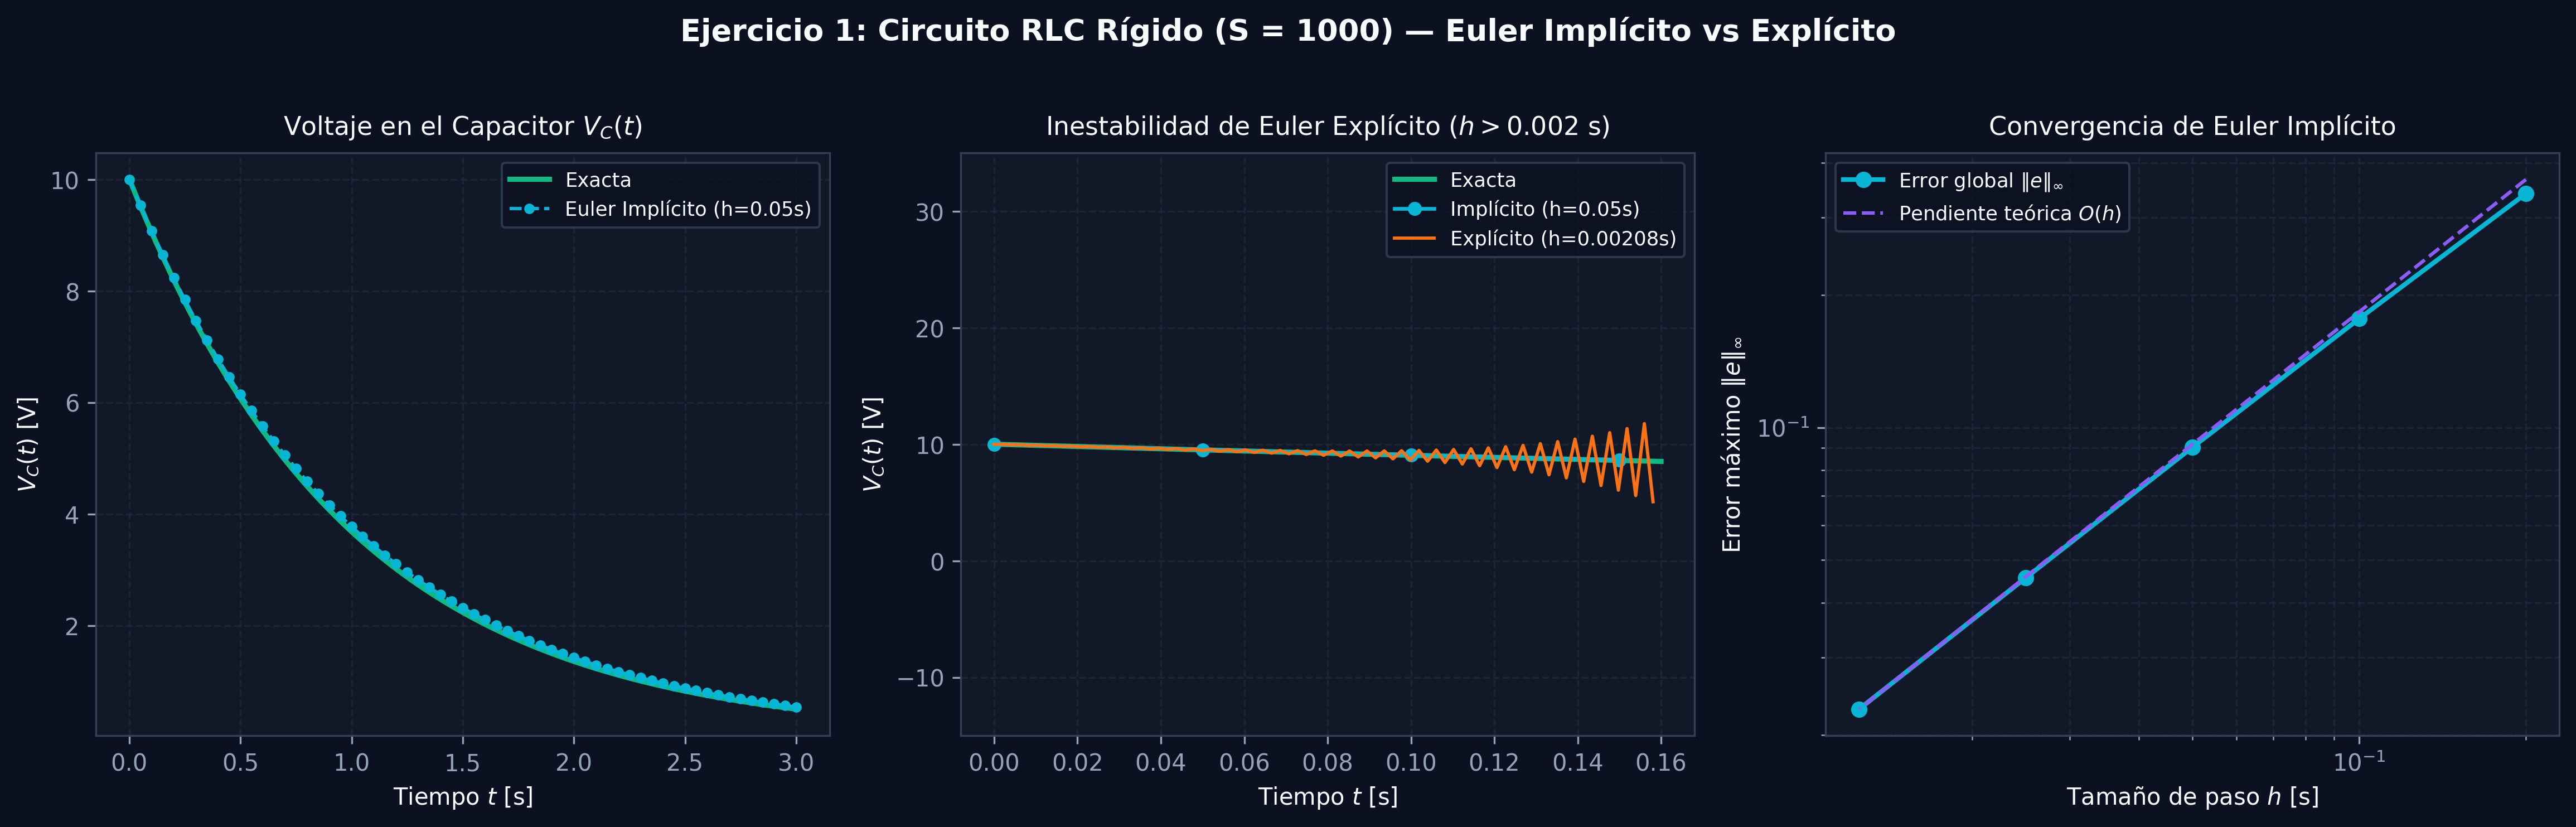
\includegraphics[width=\linewidth]{img/ej1_rlc_comparacion.png}
    \caption{Respuesta temporal, contraste de inestabilidad de Euler Explícito y curva de convergencia $O(h)$ para el circuito RLC rígido. Animación complementaria en \texttt{img/ej1\_rlc\_animacion.gif}.}
    \label{fig:ej1_rlc}
\end{figure}

% ============================================================================
% SECCIÓN 4
% ============================================================================
\section{Experimento 2: Cinética Química en Cadena $A \to B \to C$ ($3\times 3$)}

Se simula una reacción consecutiva en un reactor con constantes cinéticas $k_1 = 0.5\text{ s}^{-1}$ y $k_2 = 100\text{ s}^{-1}$ (especie intermedia $B$ de vida ultracorta, $S = 200$):
\begin{equation}
    \frac{d}{dt}\begin{pmatrix} A \\ B \\ C \end{pmatrix} =
    \begin{pmatrix} -0.5 & 0 & 0 \\ 0.5 & -100 & 0 \\ 0 & 100 & 0 \end{pmatrix}
    \begin{pmatrix} A \\ B \\ C \end{pmatrix}, \qquad \mathbf{y}(0) = \begin{pmatrix} 1 \\ 0 \\ 0 \end{pmatrix}.
\end{equation}
Para $h = 0.05\text{ s}$ (superior al límite explícito $h_{\max} = 0.02\text{ s}$), Euler Explícito genera concentraciones negativas no físicas en $[B](t)$. En contraste, Euler Implícito obtiene un error global $\|\mathbf{e}\|_\infty = 4.574 \times 10^{-3}\text{ mol/L}$, preserva estrictamente la positividad ($\min [B](t) = 0$) y conserva la masa total $|A+B+C-1| \le 3.55 \times 10^{-15}$ (precisión de máquina).

\begin{figure}[!htbp]
    \centering
    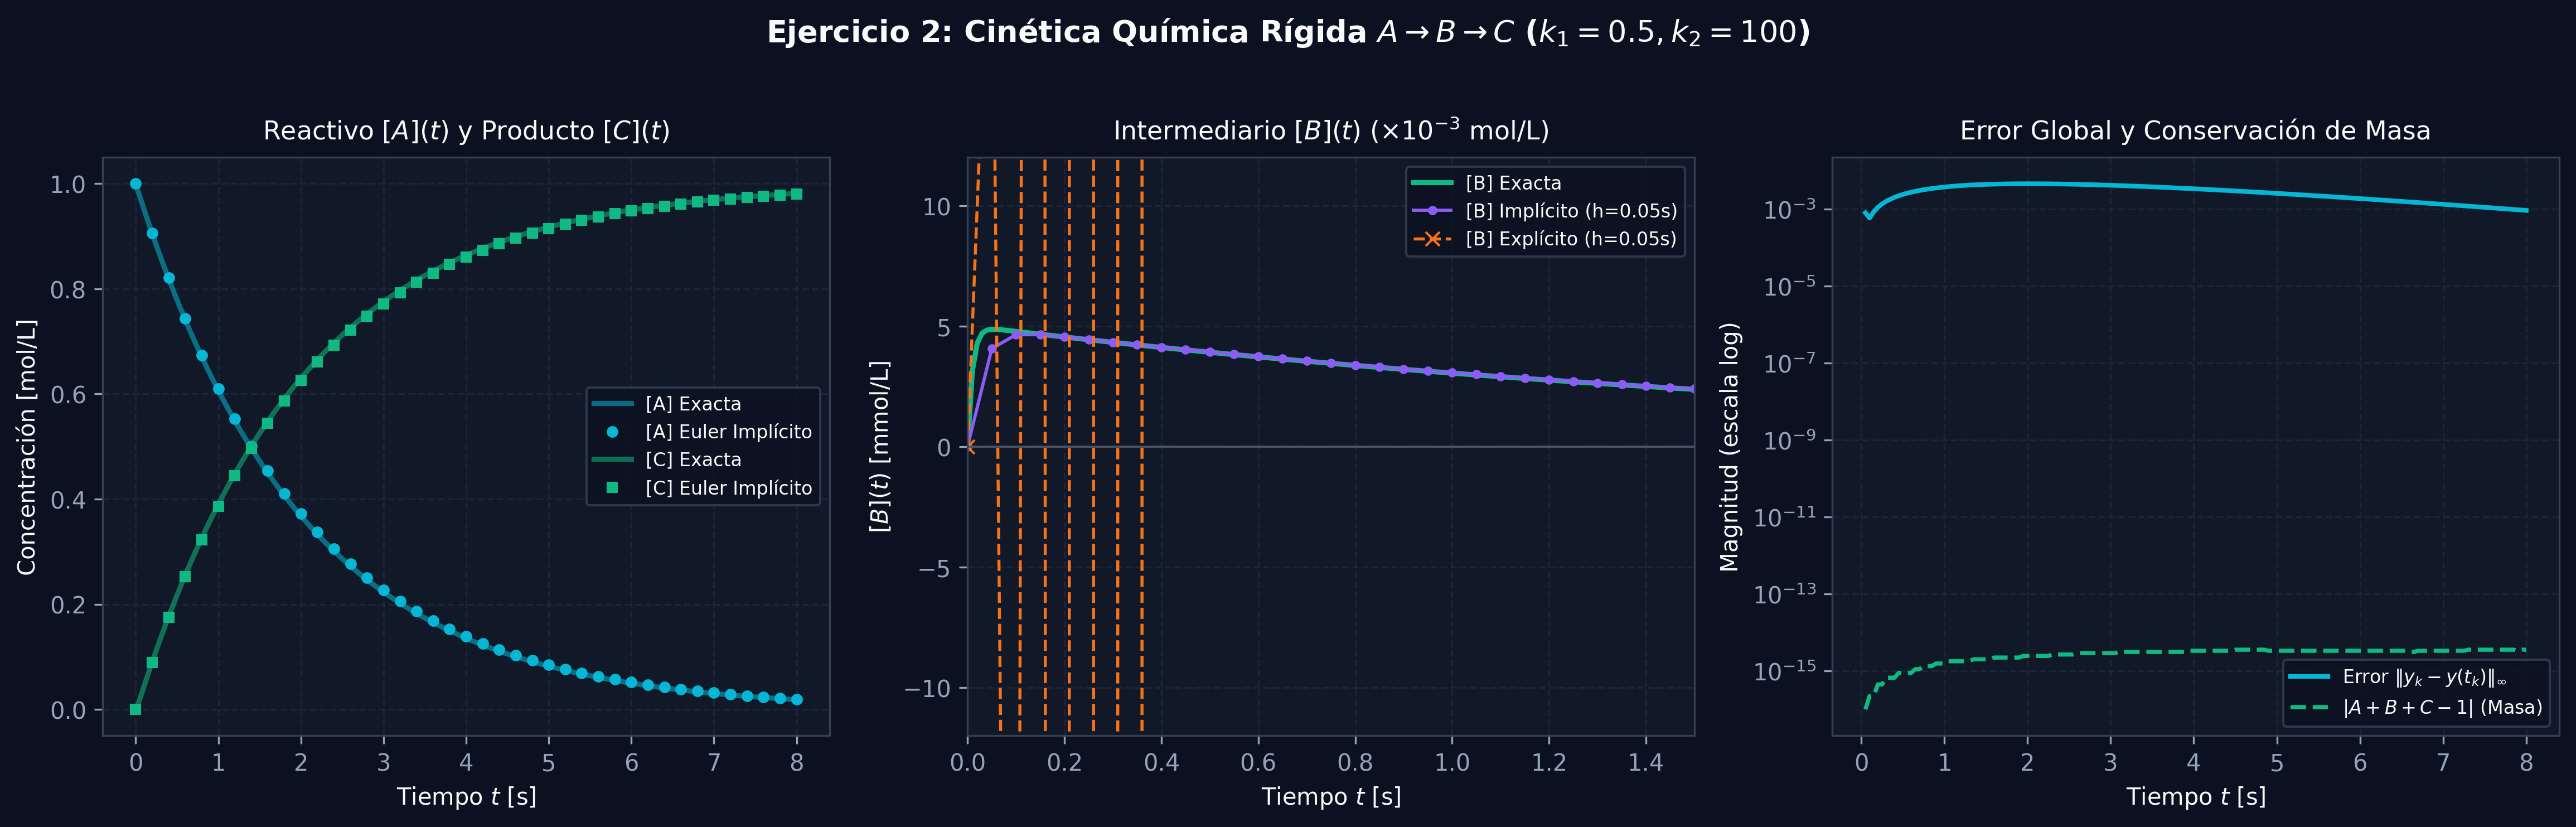
\includegraphics[width=\linewidth]{img/ej2_cinetica_quimica.png}
    \caption{Evolución de concentraciones $[A]$, $[B]$ y $[C]$, contraste de estabilidad en el intermediario y conservación de masa. Animación del reactor en \texttt{img/ej2\_cinetica\_animacion.gif}.}
    \label{fig:ej2_cinetica}
\end{figure}

% ============================================================================
% SECCIÓN 5
% ============================================================================
\section{Experimento 3: Dinámica Sísmica de Edificio de 2 Pisos ($4\times 4$)}

Para evaluar el desempeño del método en sistemas no homogéneos con modos vibratorios complejos, se modela un edificio de 2 pisos ($m_1=m_2=1$, $k_1=120$, $k_2=80$, $c_1=6$, $c_2=4$) excitado por una aceleración sísmica amortiguada $a_g(t) = 12 e^{-0.4t}\sin(4.5t)$:
\begin{equation}
    \mathbf{y}'(t) = \begin{pmatrix}
        0 & 0 & 1 & 0 \\
        0 & 0 & 0 & 1 \\
        -200 & 80 & -10 & 4 \\
        80 & -80 & 4 & -4
    \end{pmatrix}\mathbf{y}(t) +
    \begin{pmatrix} 0 \\ 0 \\ -a_g(t) \\ -a_g(t) \end{pmatrix}, \qquad \mathbf{y} = \begin{pmatrix} x_1 \\ x_2 \\ v_1 \\ v_2 \end{pmatrix}.
\end{equation}

\begin{table}[!htbp]
    \centering
    \caption{Factores de amplificación por modo propio en el edificio de 2 pisos para $h = 0.06\text{ s}$.}
    \begin{tabularx}{\linewidth}{Xrrl}
        \toprule
        \textbf{Valor propio $\lambda_i$} & \textbf{$|1 + h\lambda_i|$ (Explícito)} & \textbf{$|1/(1-h\lambda_i)|$ (Implícito)} & \textbf{Diagnóstico} \\
        \midrule
        $-6.0000 \pm 14.2829i$ & 1.0696 ($>1$) & 0.6221 ($<1$) & Explícito diverge \\
        $-1.0000 \pm 6.2450i$  & 1.0119 ($>1$) & 0.8895 ($<1$) & Explícito diverge \\
        \bottomrule
    \end{tabularx}
    \label{tab:sismo_modos}
\end{table}

Con $h = 0.06\text{ s}$, Euler Explícito inyecta energía numérica artificial y el desplazamiento del piso 2 diverge hasta $24.02\text{ m}$. Euler Implícito mantiene la estabilidad energética y estructural en todo el intervalo $[0, 8]\text{ s}$, con un error máximo en $x_2(t)$ de $0.158\text{ m}$ respecto a la referencia de alta precisión (\texttt{Radau}).

\begin{figure}[!htbp]
    \centering
    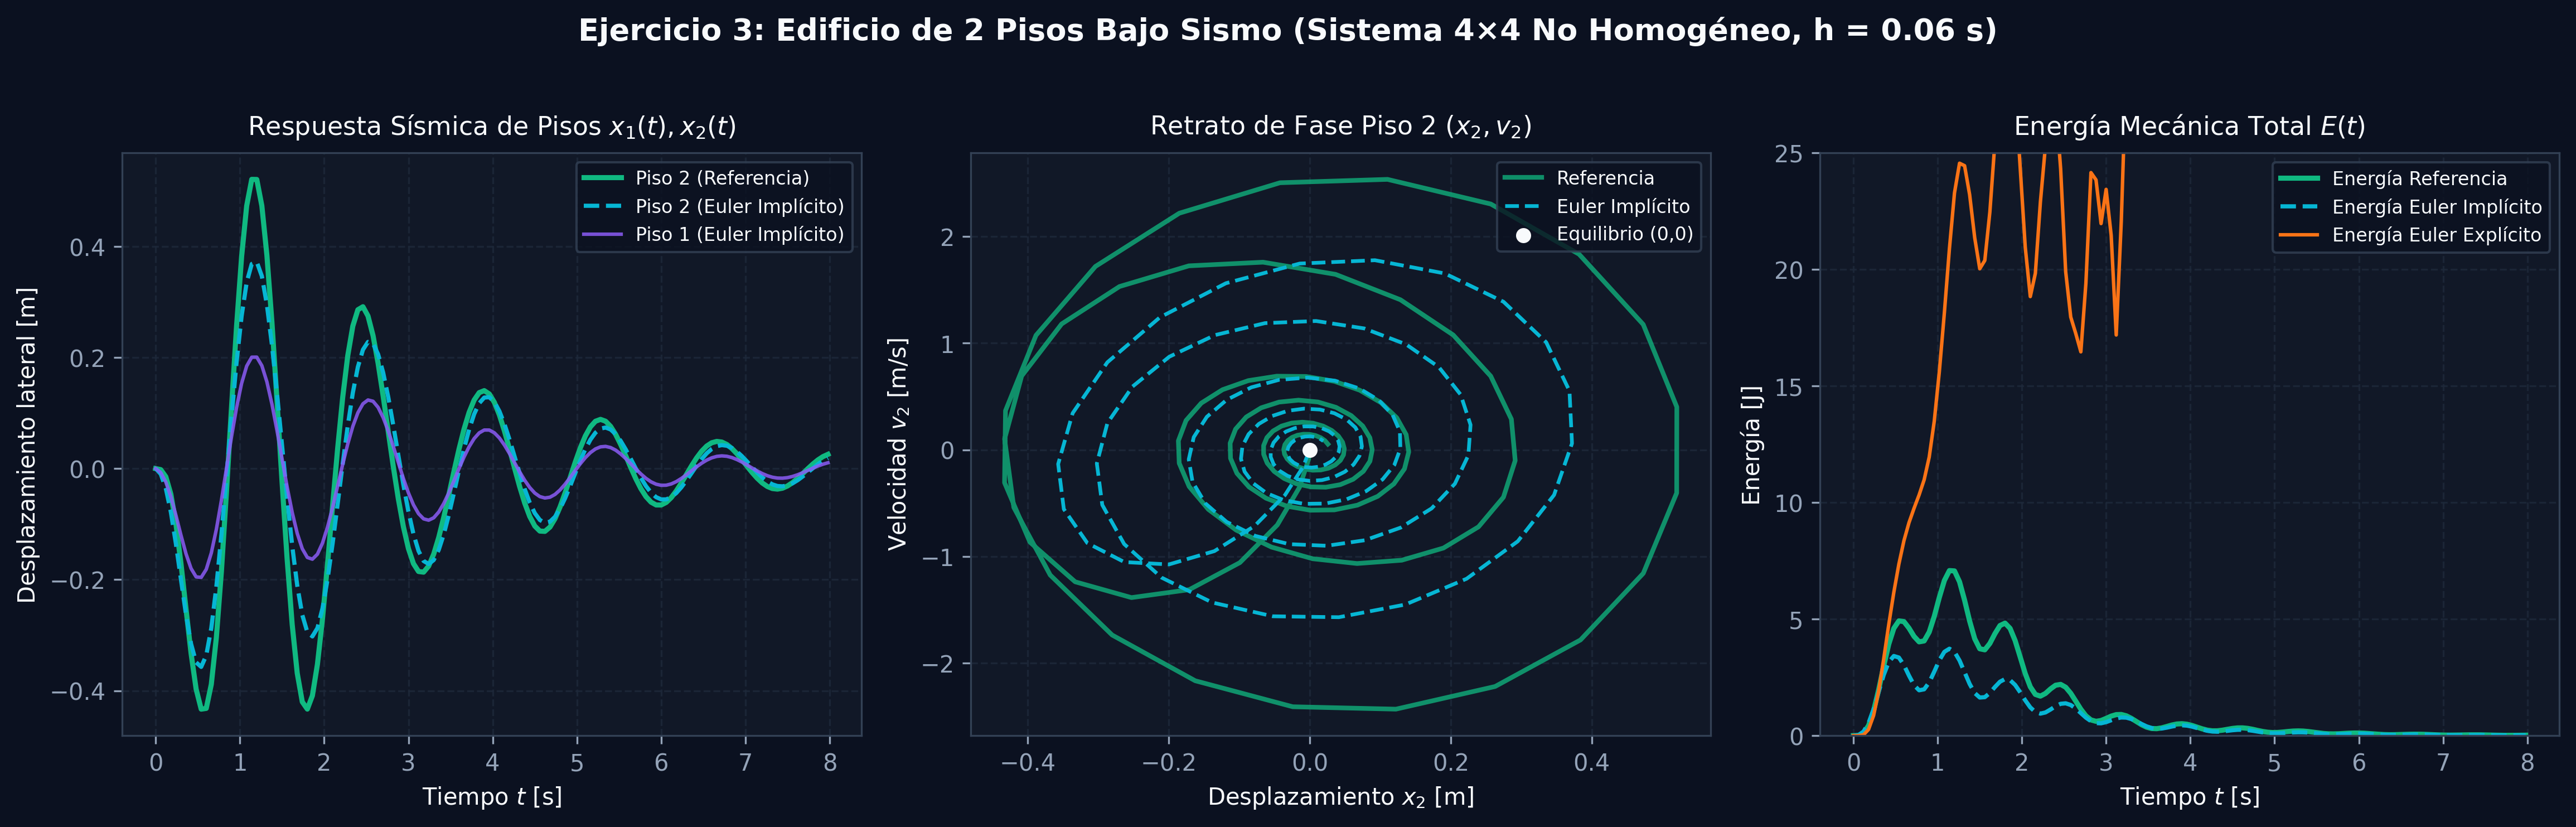
\includegraphics[width=\linewidth]{img/ej3_edificio_sismo.png}
    \caption{Respuesta sísmica de ambos pisos, retrato de fase $(x_2, v_2)$ y balance de energía mecánica. Animación 2D del edificio en \texttt{img/ej3\_edificio\_animacion.gif}.}
    \label{fig:ej3_sismo}
\end{figure}

% ============================================================================
% SECCIÓN 6
% ============================================================================
\section{Arquitectura del Dashboard Interactivo (\textit{EulerLab})}

El proyecto se complementa con la especificación técnica (\texttt{agent.md}) y visual (\texttt{design.md}) para implementar un dashboard interactivo en Python (\textbf{Streamlit + Plotly}) mediante Google Antigravity:
\begin{itemize}
    \item \textbf{Menú lateral izquierdo colapsable y fijable:} Permite ocultar la barra de navegación para ampliar el lienzo de gráficas o mantenerla fija durante el ajuste de parámetros.
    \item \textbf{Laboratorio de Estabilidad Interactivo:} Grafica el plano complejo $z = h\lambda$ y desplaza los valores propios en tiempo real al modificar el paso $h$.
    \item \textbf{Integración con \texttt{img/}:} Centraliza las gráficas estáticas (300 DPI) y animaciones \texttt{.gif} generadas por los tres scripts, además de permitir exportar nuevas simulaciones.
\end{itemize}

% ============================================================================
% SECCIÓN 7
% ============================================================================
\section{Conclusiones}

\begin{enumerate}
    \item El Método de Euler Implícito elimina la restricción severa de estabilidad de los esquemas explícitos en sistemas lineales rígidos, permitiendo pasos decenas de veces mayores que $h_{\max}$ sin divergencia.
    \item El uso de factorización LU precomputada convierte el costo de resolver $(I - hA)\mathbf{y}_{k+1} = \mathbf{y}_k + h\mathbf{g}(t_{k+1})$ en una operación $O(n^2)$ por paso, altamente eficiente en Python con SciPy.
    \item Los tres casos de estudio (RLC rígido, cinética química $A \to B \to C$ y dinámica sísmica de 2 pisos) confirmaron empíricamente el orden de convergencia $O(h)$, la conservación de masa a precisión de máquina y la estabilidad energética ante modos complejos.
\end{enumerate}

\begin{thebibliography}{9}
    \bibitem{burden2017}
    R. L. Burden, J. D. Faires y A. M. Burden, \textit{Análisis Numérico}, 10.\textsuperscript{a} ed., Cengage Learning, 2017.
    \bibitem{chapra2015}
    S. C. Chapra y R. P. Canale, \textit{Métodos Numéricos para Ingenieros}, 7.\textsuperscript{a} ed., McGraw-Hill, 2015.
    \bibitem{hairer1996}
    E. Hairer y G. Wanner, \textit{Solving Ordinary Differential Equations II: Stiff and Differential-Algebraic Problems}, 2.\textsuperscript{a} ed., Springer, 1996.
\end{thebibliography}

\end{document}
